% ПЛАН
%# Глава 3 – Численные методы для нахождение оптимальной несмещенной оценки параметров гармоник
%
%Выводы по главе:
%
%- Методы, основанные на интерполировании смежных гармоник, позволяют достичь высокой точности, во многих случаях достаточной для практического применения, однако они не позволяют достичь точности оптимальной несмещенной оценки.
%- Можно выделить два подхода к построению алгоритмов на основе корреляционного анализа: использование итерационного процесса для нахождения частоты, амплитуды и фазы каждой гармоники и использование техники дополнения нулями сигнала с целью уплотнения гармоник в спектре сигнала. Оба метода требуют существенно больших вычислительных ресурсов, чем методы основанные на интерполировании, но обеспечивают оптимальную несмещенную оценку.
%- Время расчета параметров гармоник многотонального сигнала с помощью техники дополнения нулями может быть существенно снижено за счет применения разряженного быстрого преобразования Фурье.
%- Реализация итерационного оптимизационного метода нахождения гармоник на основе чисел Фиббоначи при небольшом числе обсчитываемых гармоник обеспечивает быстродействие, близкое к итерационным методам. 
%- Реализация метода дополнение нулями сигнала при использовании разряженного преобразования Фурье имеет быстродействие менее чем на порядок худшее, чем итерационные методы, при этом быстродействие не зависит от числа обсчитываемых гармоник. Также нужно отметить больший объем памяти, требуемый для этого метода, который при этом не является критичным для современных вычислительных устройств.
%


\chapter{Численные методы для нахождения оптимальной несмещенной оценки параметров гармоник}\label{ch:ch3}

\section{Метод корреляционных функций} \label{sec:ch3/sect1}

\begin{figure}[ht]
	\centering
	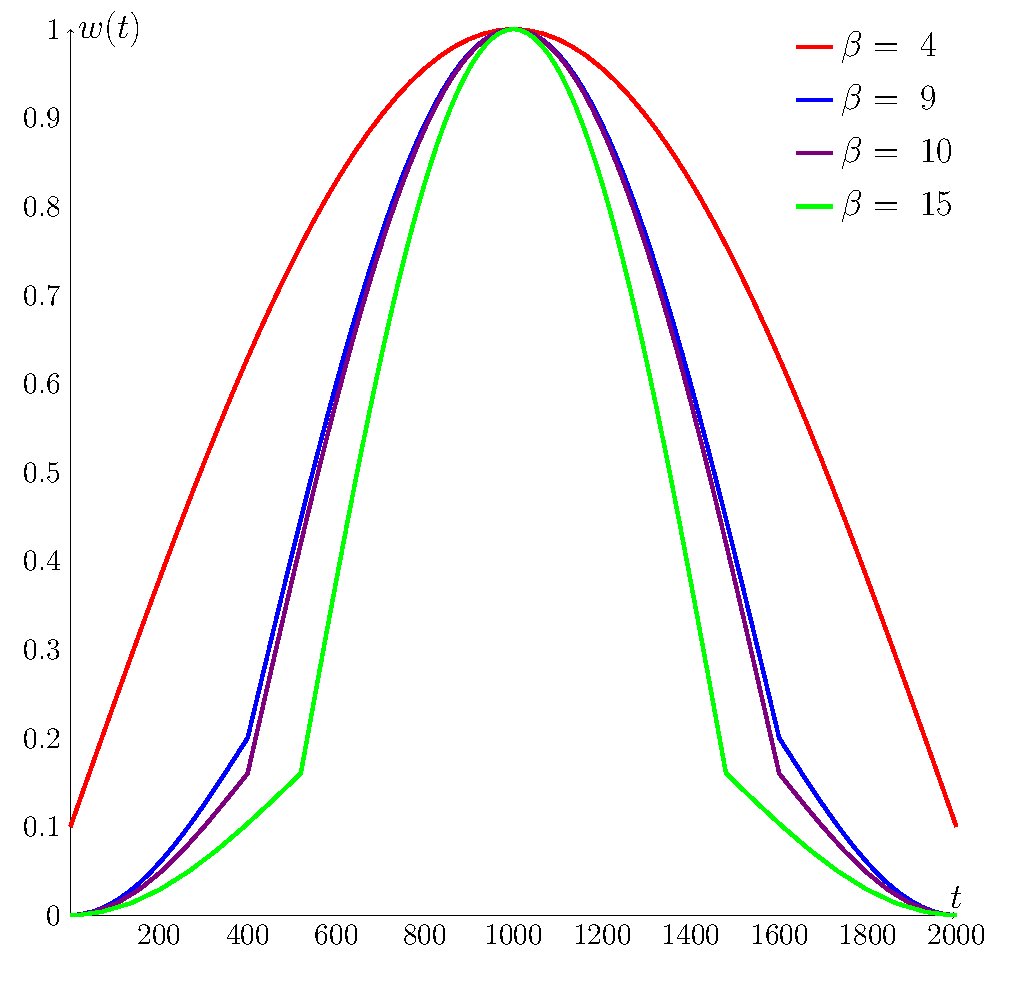
\includegraphics [scale=0.6] {Kaiser window}
	\caption{Окно Кайзера.}
	\label{img:picture23}
\end{figure}

\section{Свертка} \label{sec:ch3/sect2}

Свертка и цифровые фильтры с конечной импульсной характеристикой (КИХ) вычисляются по формуле [1]:
% 1.	Макклеллан Дж. Х., Рейдер Ч.М. Применение теории чисел в цифровой обработке сигналов.: Радио и связь, 1983. 263 с.

\begin{equation}
	\label{eq:y(n)}
	y(n) = \sum_{k=0}^{L-1}x(n-k)h(k)
\end{equation}

где $x(n)$ -- входной сигнал;

$y(n)$ -- выходной сигнал; 

$N$ -- длина сигнала x;

$h(n)$ -- импульсный отклик системы, длиной $L$. 

В случае, если длина выходного сигнала $y(n)$,  рассчитанная по формуле (1), равна $(N+L-1)$ и для его вычисления по формуле (1) требует $N*L$ умножений и $(N-1)(L-1)$ сложений. 
Недостаток вычисления операции дискретной свертки по формуле (1), заключается в том, что требуется много вычислительных операций. Другой недостаток, что происходят временные задержки при обработке последовательности, поэтому используют секционирование сигнала и вычисление свертки для его блоков.
Для решения поставленной задачи рассмотрим быстрые алгоритмы. Любой алгоритм можно описывать через соотношение между входом и выходом, либо детально предоставить информацию, объясняя его внутреннюю структуру. Если считать, что заданный алгоритм вход-выход  имеет возможность  быть описанным математической формулой, то такая реализация будет называться прямой. К быстрым алгоритмам относятся вычислительные процедуры, которые не являются очевидным способом вычисления к данному входу, основное их преимущество – сокращение количества операций.  Для оценки сложности алгоритма используют количество арифметических операций (сложения, вычитания, умножение, деление). Важно различать быстрый алгоритм, функцию, которую он вычисляет, и приложение в котором используется. Например, необходимо различать дискретное преобразование Фурье (ДПФ) от быстрого преобразования Фурье (БПФ), т.~к.  второе преобразование является  алгоритмом для первого [2]. 
% 2.	Блейхут Р. Быстрые алгоритмы цифровой обработки сигналов: Пер. с англ.–М.: Мир, 1989.–448 с.

Существует два подхода для вычисления свертки. Первый подход заключается в том, что входные последовательности x и y разбиваются на короткие секции(блоки) из несколько сотен отчетов. На выходе секции(блоки) обрабатываются поочередно методом циклической свертки. Следующий вид первого подхода заключается в вычислении циклической свертки алгоритмом Быстрого Преобразования Фурье или другими преобразованиями [2,4,5,6].

%2.	Блейхут Р. Быстрые алгоритмы цифровой обработки сигналов: Пер. с англ.–М.: Мир, 1989.–448 с.
%3.	Mou Z.J. Fast FIR filtering: algorithms and implementations / Z.J. Mou, P. Duhame // Signal Processing. – 1987. – Vo1. 13, № 4. – P. 377–384 с.
%4.	Рабинер Л. Теория и применение цифровой обработки сигналов / Л. Рабинер, Б. Гоулд. – М.: Мир, 1978. –848 с.
%5.	Нуссбаумер Г. Быстрое преобразование Фурье и алгоритмы вычисления сверток. – М.: Радио и связь, 1985.–248 с.
%6.	Оппенгейм А., Шафер М. Цифровая обработка сигналов. –М.: Техносфера, 2012 1048 с.

Второй подход, когда входные последовательности x и y  разбиваются на последовательности из четных и нечетных отчетов. Вычисление коротких последовательностей происходит быстрее. [3].
%3.	Mou Z.J. Fast FIR filtering: algorithms and implementations / Z.J. Mou, P. Duhame // Signal Processing. – 1987. – Vo1. 13, № 4. – P. 377–384 с.
Исследования для алгоритмов одномерной свертки производились в  среде разработке JetBrains CLion 2018.1 для языка программирования С. CLion – это интегрированная среда разработки (IDE), которая использует набор инструментов Cygwin (Unix-подобная среда и интерфейс командной строки для Microsoft Windows). 
В результате исследования быстродействия алгоритмов одномерной свертки на языке программирования С был получен график временных затрат с зависимостью длины фильтра от времени. Исходные данные: количество отчетов при изменении длины фильтра $100-900$ и длины сигнала $10000-40000$, количество опытов $10000$ раз. Быстродействие алгоритмов свертки на языке программирования С приведено на 
рисунке 1. 
Полученные графики построены с помощью библиотеки Matplotlib, которая строит высококачественные графики в Python. Данные графики были построены из табличных значений, формат файлов CSV (Comma-Separated Values). Режим Full возвращает свертку с выходной формой $N+L-1$.  $N$ и $L$ – размер одномерных входных массивов.

\begin{figure}[ht]
	\centering
	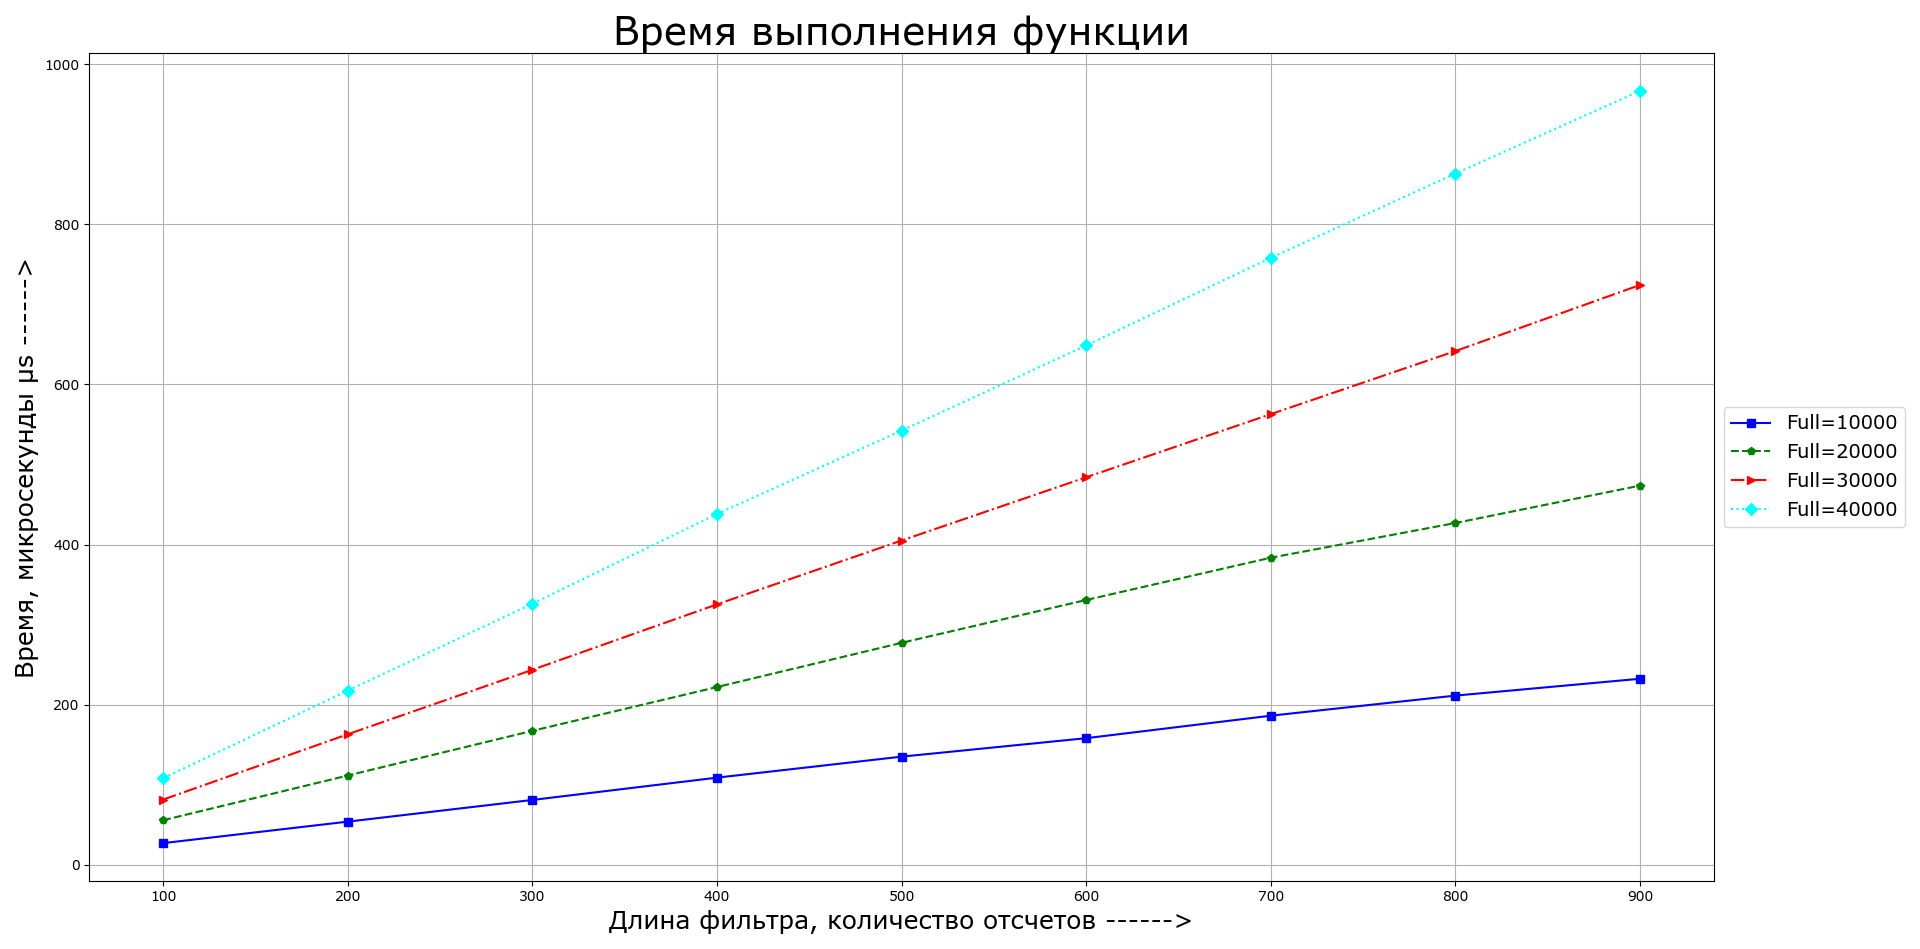
\includegraphics [scale=0.3] {convolution}
	\caption{Временные затраты на вычисление по алгоритму одномерной свертки на языке С (процессор Intel® Core™ $i5-3550$).}
	\label{img:convolution}
\end{figure}



В исследовании произведен анализ быстродействия реализаций алгоритмов одномерной свертки и цифровых фильтров. Для фильтрации  узкополосных сигналов требуются фильтры с импульсной характеристикой, содержащих большое число отчетов. 
В результате исследования была установлена необходимость минимизировать вычислительные затраты для цифровых фильтров с конечной импульсной характеристикой (рисунок 1).
Для фильтрации  узкополосных сигналов, необходимо использовать быстрые алгоритмы, т.~к. они позволяют сократить количество операций. 


\section{Интерполированный алгоритм ДПФ} \label{sec:ch3/sect3}
Интерполированный алгоритм ДПФ (IpDFT -- Interpolated Discrete Fourier Transform) является одним из наиболее широко изученных методов оценки \cite{santamaria2000comparative ,zhang2001algorithm, qian2007interharmonics, ferreira2005accurate, xie1996nonlinear, luo2015phase, jain1979high, grandke1983interpolation, andria1989windows, offelli1989interpolation, agrez2002weighted, jacobsen2007fast, belega2009multifrequency, belega2010accuracy, duda2011dft, schoukens1992interpolated}. 
% [156.-Santamaria I., Pantaleon C., Ibanez J. A comparative study of high-accuracy frequency estimation methods //Mechanical Systems and Signal Processing. – 2000. – Т. 14. – №. 5. – С. 819-834.]

% [157.-Zhang F., Geng Z., Yuan W. The algorithm of interpolating windowed FFT for harmonic analysis of electric power system //IEEE transactions on power delivery. – 2001. – Т. 16. – №. 2. – С. 160-164.]

%[158.-Qian H., Zhao R., Chen T. Interharmonics analysis based on interpolating windowed FFT algorithm //IEEE Transactions on Power Delivery. – 2007. – Т. 22. – №. 2. – С. 1064-1069.]

%[159.	Ferreira A., Sinha D. Accurate and robust frequency estimation in the ODFT domain //IEEE Workshop on Applications of Signal Processing to Audio and Acoustics, 2005. – IEEE, 2005. – С. 203-206.]

%[160.-Xie M., Adams D. F. A nonlinear finite element analysis for composite materials //Finite elements in analysis and design. – 1996. – Т. 22. – №. 3. – С. 211-223.]

%[161.-Luo J., Xie M. Phase difference methods based on asymmetric windows //Mechanical Systems and Signal Processing. – 2015. – Т. 54. – С. 52-67.]

%[162.-Jain V. K., Collins W. L., Davis D. C. High-accuracy analog measurements via interpolated FFT //IEEE Transactions on Instrumentation and Measurement. – 1979. – Т. 28. – №. 2. – С. 113-122.]

% [163.-Grandke T. Interpolation algorithms for discrete Fourier transforms of weighted signals //IEEE transactions on instrumentation and measurement. – 1983. – Т. 32. – №. 2. – С. 350-355.]

%[164.-Andria G., Savino M., Trotta A. Windows and interpolation algorithms to improve electrical measurement accuracy //IEEE Transactions on Instrumentation and Measurement. – 1989. – Т. 38. – №. 4. – С. 856-863.]

%[165.-Offelli C., Petri D. Interpolation techniques for real-time multifrequency waveform analysis //6th IEEE Conference Record., Instrumentation and Measurement Technology Conference. – IEEE, 1989. – С. 325-331.]

%[166.-Agrez D. Weighted multipoint interpolated DFT to improve amplitude estimation of multifrequency signal //IEEE Transactions on Instrumentation and Measurement. – 2002. – Т. 51. – №. 2. – С. 287-292.]

%[167.-Jacobsen E., Kootsookos P. Fast, accurate frequency estimators [DSP Tips & Tricks] //IEEE Signal Processing Magazine. – 2007. – Т. 24. – №. 3. – С. 123-125.]

%[168.	Belega D., Dallet D. Multifrequency signal analysis by interpolated DFT method with maximum sidelobe decay windows //Measurement. – 2009. – Т. 42. – №. 3. – С. 420-426.]

%[169.-Belega D., Dallet D., Petri D. Accuracy of sine wave frequency estimation by multipoint interpolated DFT approach //IEEE Transactions on Instrumentation and Measurement. – 2010. – Т. 59. – №. 11. – С. 2808-2815.]

%[170.-Duda K. DFT interpolation algorithm for Kaiser–Bessel and Dolph–Chebyshev windows //IEEE Transactions on Instrumentation and Measurement. – 2011. – Т. 60. – №. 3. – С. 784-790.]

%[171.-Schoukens J., Pintelon R., Van Kamme H. The interpolated fast Fourier transform: A comparative study //[1991] Conference Record. IEEE Instrumentation and Measurement Technology Conference. – IEEE, 1991. – С. 358-364.]


Рассмотрим непрерывный сигнал с аддитивным белым шумом:
\begin{equation}
	\label{eq:$x(t)$}
	x(t) = A_0 \cos \big( 2 \pi f_0 t + \theta_0 + e(t)\big) 
\end{equation}

где $A_0$ -- амплитуда;

$f_0$ -- частота;

$\theta_0$ -- фазовый угол;

$t$ -- время;

$e(t)$ -- белый шум. 

Частота $f_s$ с интервалом $N\bigtriangleup t$, где $\bigtriangleup t = \cfrac{1}{f_s}$, $N$ -- отчеты.

По теореме Котельникова (в зарубежной литературе теорема Найквиста -- Шеннона или теорема отчетов) непрерывные и дискретные сигналы $x(t)$ состоящих из частот ($0$ до $f_0$) можно передавать с любой точностью при помощи чисел, следующих друг за другом через $\frac{1}{2f_0}$. 

\begin{equation}
	\label{eq:$x(n)$}
	x(n) = A_0 \cos(2 \pi \frac{f_0}{f_s} n + \theta_0) + e(n), n = 0,1, \cdots , N-1
\end{equation}

По теореме Котельникова, $f_s$ больше $2f_0$. Разрешающая способность по частоте $\bigtriangleup f = \cfrac{f_s}{N}$ определяется:

\begin{equation}
	\label{eq:equation14}
	\frac{f_0}{f_s}=\frac{\lambda_0}{N}
\end{equation}

$\lambda_0$ -- количество циклов или нормированная частота.


Умножим отчеты сигнала $x(n)$ на значение окна данных $\omega(n)$.

\begin{equation}
	\label{eq:equation15}
	x_\omega(n)=A_0 \cos(\frac{2 \pi \lambda_0 n}{N}+\theta_0)\omega(n)
\end{equation}

ДПФ взвешенного сигнала может быть вычислена путем:

\begin{equation}
	\label{eq:equation16}
	X_\omega(k) = \sum_{n=0}^{N-1} x_\omega(n) e^{-j \frac{2 \pi}{N}nk}
\end{equation}

Применение \labelcref{eq:equation16} к отчетам в \labelcref{eq:equation15} дает вид:

\begin{equation}
	\label{eq:equation17}
	X_\omega(k) = \frac{A_0}{2} e^{j\phi_0}W_N(k-\lambda_0)+\frac{A_0}{2}e^{j\phi_0}W_N(k+\lambda_0)
\end{equation}

где $W_N (k)$ -- дискретное временное преобразование Фурье (DTFT-- Discrete time Fourier transform) весовой функции. 

Нормированная частота $\lambda_0$ находится между двумя самыми большими спектральными линиями. Следовательно, $\lambda_0$  может быть записано с целой частью $l_\omega$ и дробной частью $\delta_\omega$ $(-0,5<\delta_{\omega}\leq0,5)$.

\begin{equation}
	\label{eq:equation18}
	\lambda_0 = l_\omega + \delta_\omega
\end{equation}

Целая часть $l_\omega$ может быть определена с помощью отношения сигнал/шум (SNR -- signal-to-noise ratio) превышает пороговое значение (приблизительно от -$18$ до –$20$ дБ) \cite{rife1974single}. 

Подстановка формулы \labelcref{eq:equation18} в \labelcref{eq:equation17}:
\begin{equation}
	\label{eq:equation19}
	\left|{X_\omega(l_\omega)} \right| = \frac{A_0}{2} \left| e^{j\phi_0}W_N(- \delta_\omega) +e^{j\phi_0}W_N(2l_\omega+\delta_\omega) \right| 
\end{equation}

Параметр $\alpha$ зависит только от выбранного окна и отклонения частоты $\delta_{\omega}$. 

\begin{equation}
	\label{eq:equation20}
	\delta_\omega = g(\alpha)
\end{equation}

Для максимальных окон распада боковых лепестков $\delta_{\omega}$ запишем как функцию от $\alpha$ в простой форме \cite{zhang2001algorithm, qian2007interharmonics, xie1996nonlinear, luo2015phase, belega2009multifrequency, belega2010accuracy}. Для других окон предлагается решение полиномиальной аппроксимации \cite{duda2011dft}. 

Рассмотрим алгоритм техники заполнения нулями. Заполнение нулями -- это метод, определяемый как добавление нулевых значений к отчетам до вычисления ДПФ. Добавленные нулевые значения обрабатываются как дополнительные отчеты, поэтому увеличивают время измерения \labelcref{eq:equation21}:

\begin{equation}
	\label{eq:equation21}
	x_{ap}(n)=
	\begin{cases}
		x_{\omega}, \leq n < N
		\\ 0, N \leq n < MN
	\end{cases}
\end{equation}

где $(M-1) \cdot N$ -- добавление нулевых значений.

Соответственно, дискретный спектр расширяется. Эта процедура приводит к более точной выборке спектра сигнала, потому что вместо $N$ спектральных отчетов $M \cdot N$. Добавление нулевых значений и вычисление более длинного ДПФ действительно увеличивает количество точек в частотной области \cite{dorf2006circuits}.

Алгоритм техники заполнения нулями не влиет на параметры спектра (отношение сигнал/шум, спектральная утечка).  Коэффициенты ДПФ по \labelcref{eq:equation21}:

\begin{equation}
	\label{eq:equation22}
	X(N)= \sum_{n=0}^{MN-1} x_{ap}(n) e^{-j \frac{2 \pi}{N}\cdot \frac{k}{M} \cdot n}, 0\leq k \leq MK-1
\end{equation}
По сравнению с \labelcref{eq:equation16} получается:

\begin{equation}
	\label{eq:equation23}
	X(k)= X_\omega \left( {\frac{k}{M}}\right)  \end{equation}
Соответственно, \labelcref{eq:equation19} можно переформулировать как:

\begin{equation}
	\label{eq:equation24}
	\left| {X(l)} \right|   = \frac{A_0}{2}\left| {e^{j\phi_0}W_N(-\delta)+e^{-j\phi_0}W_N \left(\frac{2l}{M}+\delta \right)} \right|,
\end{equation}

где $l$ и $\hat{\delta}
\left( {\delta= \frac{\hat{\delta}}{M}}\right) $
часть для $M\lambda_0$. Точно так же $l$ возвращается максимальной процедурой поиска X(k). На этом этапе три крупнейших линии $X(k)$ даны $\left| {X(l)} \right|$,$\left| {X(l+1)} \right|$ а также $\left|{X(l-1)}\right|$.

Рассмотрим алгоритм интерполяции для окна Хеннинга с техникой заполнения нулями.
Если $\lambda_0$ удовлетворяет $5<\lambda_0$ , а также $\lambda_0 < \frac{N}{2}-5$, тогда помехи от второго слагаемого могут быть минимальными и ими можно пренебречь. Поэтому \labelcref{eq:equation24} сводится к:
\begin{equation}
	\label{eq:equation25}
	\left| {X(l)} \right| \cong \frac{A_0}{2}\left| {W_N(-\delta)} \right|,
\end{equation}

Если $\left| {X(l)} \right| \cong \frac{A_0}{2}\left| {W_N(\varepsilon -\delta)} \right|$ и $\left| {X(l-1)} \right| \cong \frac{A_0}{2} \left| {W_N(\varepsilon +\delta)} \right|$, где $\varepsilon=\frac{1}{M}$. 

Для окна Хеннинга (Hanning window), $W_N (k) \cong \frac{sin(\pi k)}{h(k)}$,
$h(k) = 2 \pi k (1-k^2)$ \cite{xie1996nonlinear}
%[160.	Xie M., Adams D. F. A nonlinear finite element analysis for composite materials //Finite elements in analysis and design. – 1996. – Т. 22. – №. 3. – С. 211-223.]

\begin{equation}
	\label{eq:equation26}
	\left| {X(l)} \right| \cong \frac{A_0}{2} \frac{\sin{(\pi \delta)} }{h(\delta)} ,
\end{equation}

\begin{equation}
	\label{eq:equation27}
	\left| {X(l+1)} \right| \cong \frac{A_0}{2} \frac{\sin{(\pi \varepsilon - \pi \delta)} }{h(\varepsilon - \delta)} ,
\end{equation}

\begin{equation}
	\label{eq:equation28}
	\left| {X(l+1)} \right| \cong \frac{A_0}{2} \frac{\sin{(\pi \varepsilon + \pi \delta)} }{h(\varepsilon + \delta)}
\end{equation}

Объединим уравнения вместе (\labelcref{eq:equation27} и \labelcref{eq:equation28}):

\begin{equation}
	\label{eq:equation29}
	h(\varepsilon+\delta)\left|{X(l-1)} \right| - h(\varepsilon-\delta) \left|{X(l+1)} \right| \cong A_0 \sin{(\pi \delta)} \cos{(\pi \varepsilon)}
\end{equation}

Дальнейшее объединение \labelcref{eq:equation26} и \labelcref{eq:equation29}

\begin{equation}
	\label{eq:equation30}
	h(\delta+\varepsilon)\left|{X(l-1)} \right| - h(\delta - \varepsilon) \left|{X(l+1)} \right| \cong 2 \left|{X(l)} \right| h(\delta) \cos{(\pi \varepsilon)}
\end{equation}

Теперь введем две переменные $\gamma_1$,$\gamma_2$ определяются как:

\begin{equation}
	\label{eq:equation31}
	\gamma_1 = \frac{\left| X(l-1)\right|}{\left| X(l)\right|}
\end{equation}

\begin{equation}
	\label{eq:equation32}
	\gamma_1 = \frac{\left| X(l+1)\right|}{\left| X(l)\right|}
\end{equation}

Для простоты и краткости будем использовать знак $«=»$ в \labelcref{eq:equation30}, вместо $\cong$. Но отношение аппроксимации остаются. 

\begin{equation}
	\label{eq:equation33}
	h(\delta +\varepsilon)\gamma_1 - h(\delta -\varepsilon)\gamma_2 = 
	2h(\delta) \cos(\pi \varepsilon) 
\end{equation}

При условии $h(\delta +\varepsilon)$,$h(\delta -\varepsilon)$ получаем:

\begin{equation}
	\label{eq:equation34}
	{a \delta}^3 + {b \delta}^2 + c \delta + d = 0, 
\end{equation}

где $a = 2 \cos(\pi \varepsilon)-(\gamma_1 + \gamma_2)$;

$b = -3(\gamma_1 - \gamma_2)\varepsilon$;

$c = \left( \gamma_1 + \gamma_2 - \frac{2 \cos(\pi \varepsilon)}{1-3\varepsilon^2}
\right) \left( {1-3\varepsilon^2} \right) $;

$d = ( \gamma_1 - \gamma_2)(\varepsilon - \varepsilon^3)$

\begin{equation}
	\label{eq:equation35}
	g(\delta) = {a \delta}^3 + {b \delta}^2 + c \delta + d
\end{equation}

Можно доказать, что $g(-1)>0$,$g(-0,5)<0$,$g(0,5)>0$,$g(1)<0$ 

\begin{equation}
	\label{eq:equation36}
	\gamma_1 = \frac{\left| X(l-1)\right|}{\left| X(l)\right|} = \frac{\sin({\pi \varepsilon + \pi \delta})}{h(\varepsilon + \delta)} \cdot \frac{h(\delta)}{\sin(\pi \delta)}
\end{equation}

\begin{equation}
	\label{eq:equation37}
	\gamma_2 = \frac{\left| X(l+1)\right|}{\left| X(l)\right|} = \frac{\sin({\pi \varepsilon - \pi \delta})}{h(\varepsilon - \delta)} \cdot \frac{h(\delta)}{\sin(\pi \delta)}
\end{equation}

где $\delta \in[-0.5,0.5]$ а также $\varepsilon\in[0,0.5]$. Согласно формуле \labelcref{eq:equation35}

\begin{equation}
	\label{eq:equation38}
	f(0,5) = -\frac{3}{4} \cos(\pi \varepsilon) + \frac{(1-4 \varepsilon^2)}{8} \left[ {\gamma_1 (3+2 \varepsilon)+\gamma_2 (3-2 \varepsilon)}\right] 
\end{equation}

\begin{equation}
	\label{eq:equation39}
	f(-0,5) = +\frac{3}{4} \cos(\pi \varepsilon) + \frac{(1-4 \varepsilon^2)}{8} \left[ {\gamma_1 (3-2 \varepsilon)+\gamma_2 (3+2 \varepsilon)}\right] 
\end{equation}

\begin{equation}
	\label{eq:equation40}
	f(1) = -\gamma_1 \varepsilon(\varepsilon+1)(\varepsilon + 2) + \gamma_2 \varepsilon(\varepsilon-1)(\varepsilon - 2)
\end{equation}

\begin{equation}
	\label{eq:equation41}
	f(-1) = -\gamma_1 \varepsilon(\varepsilon-1)(\varepsilon - 2) + \gamma_2 \varepsilon(\varepsilon+1)(\varepsilon + 2)
\end{equation}

Определяем $p(\delta)$:

\begin{equation}
	\label{eq:equation42}
	p(\delta) = \gamma_1 (3+2\varepsilon) + \gamma_2 (3-2\varepsilon)
\end{equation}

Определяем $q(\delta)$:
\begin{equation}
	\label{eq:equation43}
	q(\delta) = \gamma_1 (3-2\varepsilon) + \gamma_2 (3+2\varepsilon)
\end{equation}

$p(\delta)$ является монотонно возрастающей функцией. Поэтому:
\begin{equation}
	\label{eq:equation44}
	p_{min}(\delta) = p(\delta = 0,5) = \frac{6 \cos(\pi  \varepsilon)}{1-4\varepsilon ^2}
\end{equation}

также
\begin{equation}
	\label{eq:equation45}
	q_{min}(\delta) = q(\delta = -0,5) = \frac{6 \cos(\pi  \varepsilon)}{1-4\varepsilon ^2}
\end{equation}

Тогда
\begin{equation}
	\label{eq:equation46}
	f(0,5) > -\frac{3}{4} \cos (\pi \varepsilon) + \frac{(1-4 \varepsilon ^2)}{8} p_{min} (\delta) = - \frac{3}{4} \cos(\pi \varepsilon) + \frac{3 \ cos(\pi \varepsilon)}{4} = 0 
\end{equation}

\begin{equation}
	\label{eq:equation47}
	f(-0,5) < \frac{3}{4} \cos (\pi \varepsilon) + \frac{(1-4 \varepsilon ^2)}{8} q_{min} (\delta) = + \frac{3}{4} \cos(\pi \varepsilon) - \frac{3 \ cos(\pi \varepsilon)}{4} = 0 
\end{equation}

Определим:
\begin{equation}
	\label{eq:equation48}
	u(\varepsilon, \gamma) = \frac{f(1)}{\varepsilon \gamma_1} = (\varepsilon ^2 + 2) (\gamma - 1) - 3\varepsilon (\gamma + 1)
\end{equation}

\begin{equation}
	\label{eq:equation49}
	\nu(\varepsilon, \gamma) = \frac{f(-1)}{\varepsilon \gamma_1} = (\varepsilon ^2 + 2) (\gamma - 1) + 3\varepsilon (\gamma + 1)
\end{equation}

$\gamma = \frac{\gamma_1}{\gamma_2}$

\begin{equation}
	\label{eq:equation50}
	u'_{\gamma}(\varepsilon, \gamma) = \varepsilon^2 - 3\varepsilon + 2 = (\varepsilon - 2)(\varepsilon -1) >0
\end{equation}

\begin{equation}
	\label{eq:equation51}
	{\nu}'_\gamma
	(\varepsilon, \gamma) = \varepsilon^2 + 3\varepsilon + 2 = (\varepsilon + 2)(\varepsilon + 1) >0
\end{equation}


\begin{equation}
	\label{eq:equation52}
	u _{max}(\varepsilon, \gamma) =
	\left( {\varepsilon^2+2} \right) 
	\left( {\frac{1,5+\varepsilon}{1,5-\varepsilon}-1} \right) - 3 \varepsilon 
	\left( {\frac{1,5+\varepsilon}{1,5-\varepsilon}+1} \right) = \frac{\varepsilon}{1,5-\varepsilon}(2\varepsilon^2 - 5) < 0
\end{equation}

\begin{equation}
	\label{eq:equation53}
	\nu _{min}(\varepsilon, \gamma) =
	\left( {\varepsilon^2+2} \right) 
	\left( {\frac{1,5-\varepsilon}{1,5+\varepsilon}-1} \right) - 3 \varepsilon 
	\left( {\frac{1,5-\varepsilon}{1,5+\varepsilon}+1} \right) = \frac{\varepsilon}{1,5-\varepsilon}(5-2\varepsilon^2) > 0
\end{equation}

Соответственно:

\begin{equation}
	\label{eq:equation54}
	f(1) = u(\varepsilon, \gamma)(\varepsilon \gamma_1) <0
\end{equation}

\begin{equation}
	\label{eq:equation55}
	f(-1) = \nu(\varepsilon, \gamma)(\varepsilon \gamma_1) > 0
\end{equation}

Согласно исследованию в \cite{nickalls1993new}, корни можно выразить:

%[174.	Nickalls R. W. D. A new approach to solving the cubic: Cardan’s solution revealed //The Mathematical Gazette. – 1993. – Т. 77. – №. 480. – С. 354-359.]

\begin{equation}
	\label{eq:equation56}
	\delta_1 = 
	\delta_0 + 2 \sigma \cos \left({\frac{2 \pi}{3}} + \varphi  \right) 
\end{equation}

\begin{equation}
	\label{eq:equation57}
	\delta_2 = 
	\delta_0 + 2 \sigma \cos \left({\frac{2 \pi}{3}} - \varphi  \right) 
\end{equation}

\begin{equation}
	\label{eq:equation58}
	\delta_3 = 
	\delta_0 + 2 \sigma \cos (\varphi) 
\end{equation}

$\delta_0 = \frac{-a}{3b};$

$\sigma = \sqrt{\frac{b^2 - 3ac}{9a^2}}$

$\cos(3 \varphi) = - g \left( {\frac{\delta_0}{p}}
\right) $

$p = -a \delta_0 ^3$

$\delta_1$ и $\delta_3$ выходят за пределы определенного диапазона $(-0,5;0,5]$. Таким образом, единственным решением является $\delta_2 $. Получаем:

\begin{equation}
	\label{eq:equation59}
	\hat{\delta} = \delta_2 + \delta_0 + 2 \sigma \cos \left({\frac{2 \pi}{3} - \varphi} \right) 
\end{equation}

Рассмотрим расширение на другие классические окна .

Расширим интерполяцию для других классических окон, используя метод подгонки основного лепестка. 

\begin{equation}
	\label{eq:equation60}
	S(k) = [W_C (k)]^q - W_H (k)
\end{equation}

где $W_C (k)$ -- обозначает нормализованный спектр любого классического окна;

$W_H (k)$ -- обозначает нормализованный спектр окна Хеннинга;

$q = \frac{S L_{Han}}{S L_\omega(n)}$

$S L_{Han}$ и $S L_\omega(n)$ -- представляют собой убывающие потери $SL$ окна Хеннинга.

Можно определить, что $|S(k)|$ очень мало 
для большинства классических окон, если $k$ находится в диапазоне  $(-0,5;0,5]$. 
Например, максимальное значение $|S(k)|$ равняется $10-5$ для окна Хемминга(Hamming window) и $10^-4$ для окна Блэкмена (Blackman window).
Означает, что $[W_C (k)]^q$, а также $W_H (k)$ хорошо сочетаются друг с другом в середине их основных лепестков. 
Подразумевается, что вышеуказанный алгоритм интерполяции может быть расширен для классических окон, пока $[W_C (k)]^q$ используется $k$ и ограничен в диапазоне $[-0,5;0,5]$. 
С техникой заполнения нулями $(M\geq3)$, три самые большие спектральные линии, которые используются в алгоритме интерполяции, легко удовлетворяют требованию. Для большого $M$, погрешность оценки будет уменьшаться как в шуме, так и в ситуации без шума. Однако улучшение не ясно, когда $(M>5)$. С другой стороны, объем расчета увеличится из-за добавленного нуля. Следовательно, учитывая объем вычислений и алгоритм БПФ для radix-2, часто выбираем $(M=4)$ для практических измерений.

Согласно определению в уравнениях \labelcref{eq:equation31} и \labelcref{eq:equation32}, имеем

\begin{equation}
	\label{eq:equation62}
	\gamma_1 = \frac{\left| X(l-1)\right|}{\left| X(l)\right|} = \frac{\sin \pi({\delta + \varepsilon})}{\sin \pi \delta} \cdot \frac{h(\delta)}{h(\delta + \varepsilon)}
\end{equation}

\begin{equation}
	\label{eq:equation63}
	\gamma_2 = \frac{\left| X(l+1)\right|}{\left| X(l)\right|} = \frac{\sin \pi({\delta - \varepsilon})}{\sin \pi \delta} \cdot \frac{h(\delta)}{h(\delta - \varepsilon)}
\end{equation}

\begin{equation}
	\label{eq:equation64}
	\gamma = \frac{\left| X(l+1)\right|}{\left| X(l-1)\right|} = \frac{\sin \pi({\delta - \varepsilon})}{\sin \pi ({\delta + \varepsilon})} \cdot \frac{h({\delta + \varepsilon})}{h(\delta - \varepsilon)}
\end{equation}

Знаем $\gamma_1$, является монотонно убывающей функцией и $\gamma_2$, $\gamma$ является монотонно возрастающей функцией в зависимости от $\delta$ в диапазоне $[-0.5;0.5]$. Итак, можем получить

\begin{equation}
	\label{eq:equation65}
	\gamma_{1 max} = \gamma_1 (\delta = - 0,5) = \frac{3 \cos \pi \varepsilon}{(1 + 2 \varepsilon)(1 - 2 \varepsilon)(3 - 2 \varepsilon)}
\end{equation}

\begin{equation}
	\label{eq:equation66}
	\gamma_{1 min} = \gamma_1 (\delta = 0,5) = \frac{3 \cos \pi \varepsilon}{(1 + 2 \varepsilon)(1 - 2 \varepsilon)(3 + 2 \varepsilon)}
\end{equation}

\begin{equation}
	\label{eq:equation67}
	\gamma_{2 max} = \gamma_2 (\delta = 0,5) = \frac{3 \cos \pi \varepsilon}{(1 + 2 \varepsilon)(1 - 2 \varepsilon)(3 - 2 \varepsilon)}
\end{equation}

\begin{equation}
	\label{eq:equation68}
	\gamma_{2 min} = \gamma_2 (\delta = -0,5) = \frac{3 \cos \pi \varepsilon}{(1 + 2 \varepsilon)(1 - 2 \varepsilon)(3 + 2 \varepsilon)}
\end{equation}

\begin{equation}
	\label{eq:equation69}
	\gamma_{max} = \gamma(\delta = 0,5) = \frac{1,5+ \varepsilon}{1,5 - \varepsilon}
\end{equation}

\begin{equation}
	\label{eq:equation70}
	\gamma_{min} = \gamma(\delta = -0,5) = \frac{1,5 - \varepsilon}{1,5 + \varepsilon}
\end{equation}

Согласно бесконечному представлению Эйлера функции синуса:

\begin{equation}
	\label{eq:equation71}
	\sin \pi \delta = \pi \delta \prod\limits_{n = 1}^\infty \left( 1- \frac{\delta^2}{n^2} \right) 
\end{equation}

\begin{equation}
	\label{eq:equation72}
	E(\delta) = \frac{\sin(\pi \delta) }{h(\delta)} = \frac{\pi \delta \prod\limits_{n = 1}^\infty \left( 1- \frac{\delta^2}{n^2}\right)}{\pi \delta (1 - \delta^2)} = \prod\limits_{n = 2}^\infty \left( 1 - \frac{\delta^2}{n^2}\right) \geq 0 
\end{equation}

Находим производную $E(\delta)$:     

\begin{equation}
	\label{eq:equation73}
	E'(\delta) = E(\delta)L(\delta)
\end{equation}

\begin{equation}
	\label{eq:equation74}
	L(\delta) = \sum_{n=2}^{\infty} \frac{-2 \delta}{n^2 - \delta^2} = \sum_{n=2}^{\infty} \left(  \frac{1}{n + \delta} -  \frac{1}{n - \delta} \right) 
\end{equation}

\begin{equation}
	\label{eq:equation75}
	D(\delta) = \frac{E(\delta)}{E(\delta + \epsilon)} = \frac{\prod\limits_{n = 2}^\infty \left( 1 - \frac{\delta^2}{n^2} \right) }{\prod\limits_{n = 2}^\infty \left( \frac{1 - (\delta + \epsilon)^2}{n^2}\right)} = \prod\limits_{n = 2}^\infty \frac{n^2 - \delta^2}{n^2 - (\delta + \epsilon)^2}
\end{equation}

\begin{equation}
	\label{eq:equation76}
	D'(\delta) = \frac{E(\delta)L(\delta)E(\delta + \epsilon) - E(\delta)E(\delta + \epsilon)L(\delta + \epsilon)}{E^2 (\delta + \epsilon)} = \frac{E(\delta) [L(\delta) - L(\delta + \epsilon)])}{E(\delta + \epsilon)}
\end{equation}

\begin{equation}
	\label{eq:equation77}
	L(\delta) - L(\delta + \epsilon) = \sum_{n=2}^{\infty} \left(  \frac{\epsilon}{(n + \delta)(n + \delta + \epsilon)} + \frac{\epsilon}{(n - \delta)(n - \delta - \epsilon)} \right) > 0
\end{equation}

\begin{equation}
	\label{eq:equation78}
	D'(\delta) > 0 
\end{equation}

$D(\delta)$ -- монотонно возрастающая функция в зависимости от $\delta$, $\frac{1}{D(\delta)}$ -- монотонно убывающая функция. 

На основании уравнения \labelcref{eq:equation72} $\gamma_1, \gamma_2$ могут быть представлены:

\begin{equation}
	\label{eq:equation79}
	\gamma_1 = \frac{E(\delta + \epsilon)}{E(\delta)} 
\end{equation}

\begin{equation}
	\label{eq:equation80}
	\gamma_2 = \frac{E(\delta - \epsilon)}{E(\delta)} 
\end{equation}

\begin{equation}
	\label{eq:equation81}
	p(\delta) = \frac{[E(\delta + \epsilon)(3 + 2 \epsilon) + E(\delta - \epsilon)(3 - 2 \epsilon)]}{E(\delta)}
\end{equation}

\begin{equation}
	\label{eq:equation82}
	q(\delta) = \frac{[E(\delta + \epsilon)(3 - 2 \epsilon) + E(\delta - \epsilon)(3 + 2 \epsilon)]}{E(\delta)}
\end{equation}

\begin{equation}
	\label{eq:equation83}
	p'(\delta) = \frac{H_{p}(\delta, \epsilon)}{E(\delta)}
\end{equation}

\begin{equation}
	\label{eq:equation84}
	q'(\delta) = \frac{H_{q}(\delta, \epsilon)}{E(\delta)}
\end{equation}

Где $H_{p}(\delta, \epsilon)$ и $H_{q}(\delta, \epsilon)$ соответственно:

\begin{equation}
	\label{eq:equation85}
	H_{p}(\delta, \epsilon) = E(\delta + \epsilon)(3 + 2 \epsilon) [L (\delta + \epsilon) - L(\delta)] + E(\delta - \epsilon)(3 - 2\epsilon) [L(\delta - \epsilon) - L(\delta)]
\end{equation}

\begin{equation}
	\label{eq:equation86}
	H_{q}(\delta, \epsilon) = E(\delta + \epsilon)(3 - 2 \epsilon) [L (\delta + \epsilon) - L(\delta)] + E(\delta - \epsilon)(3 + 2\epsilon)[L(\delta - \epsilon) - L(\delta)]
\end{equation}

\begin{equation}
	\label{eq:equation87}
	H_{p}(\delta, \epsilon) + H_{p}(- \delta, \epsilon) = 4 \epsilon E (\delta + \epsilon) [L(\delta + \epsilon) - L(\delta)] + 4 \epsilon E (\delta - \epsilon)[L(\delta) - L (\delta - \epsilon)] 
\end{equation}

\begin{equation}
	\label{eq:equation88}
	H_{q}(\delta, \epsilon) + H_{q}(- \delta, \epsilon) = - 4 \epsilon E (\delta + \epsilon) [L(\delta + \epsilon) - L(\delta)] - 4 \epsilon E (\delta - \epsilon)[L(\delta) - L (\delta - \epsilon)]  
\end{equation}

Если $L (\delta - \epsilon) - L(\delta) < 0$ и $L(\delta) - L(\delta - \epsilon) < 0$, то:

\begin{equation}
	\label{eq:equation89}
	H_{p}(\delta, \epsilon) + H_{p}(- \delta, \epsilon) < 0  
\end{equation}

\begin{equation}
	\label{eq:equation90}
	H_{q}(\delta, \epsilon) + H_{q}(- \delta, \epsilon) > 0  
\end{equation}

\begin{equation}
	\label{eq:equation91}
	H_{p}(\delta, \epsilon) < 0
\end{equation}

\begin{equation}
	\label{eq:equation92}
	H_{q}(\delta, \epsilon) > 0
\end{equation}

\begin{equation}
	\label{eq:equation93}
	p'(\delta) = \frac{H_{p}(\delta, \epsilon)}{E(\delta)} < 0
\end{equation}

\begin{equation}
	\label{eq:equation94}
	q'(\delta) = \frac{H_{q}(\delta, \epsilon)}{E(\delta)} > 0
\end{equation}

где $p(\delta)$ -- убывающая функция;

$\delta$ -- убывающая функция;

$q(\delta)$ -- возрастающая функция.

\begin{equation}
	\label{eq:equation95}
	I(\delta, \epsilon) = \frac{E(\delta - \epsilon)}{E(\delta + \epsilon)} \cdot \frac{L(\delta - \epsilon) - L(\delta)}{L(\delta) - L(\delta + \epsilon)}
\end{equation}

\begin{equation}
	\label{eq:equation96}
	K(\epsilon) = \frac{3 + 2\epsilon}{3 - 2\epsilon}
\end{equation}

Если $I(\delta, \epsilon) > 0$, $0 < K(\epsilon) < 1 < K (\epsilon)$, а также $K(- \epsilon)K(\epsilon) = 1$.

\begin{equation}
	\label{eq:equation97}
	\frac{H_{p}(\delta, \epsilon)}{H_{p}(- \delta, \epsilon)} = \frac{I(\delta, \epsilon) - K(\epsilon)}{K(- \epsilon) - I(\delta, \epsilon)}
\end{equation}

\begin{equation}
	\label{eq:equation98}
	\frac{H_{q}(\delta, \epsilon)}{H_{q}(- \delta, \epsilon)} = \frac{K(- \epsilon) -  I(\delta, \epsilon)}{I(\delta, \epsilon) - K(\epsilon)}
\end{equation}

Если $\delta > 0$, то:
\begin{equation}
	\label{eq:equation99}
	K(- \epsilon) < \frac{E(\delta + \epsilon)}{E(\delta - \epsilon)}
\end{equation}

\begin{equation}
	\label{eq:equation100}
	1 < \frac{L(\delta) - L(\delta + \epsilon)}{L(\delta - \epsilon) - L(\delta)} < K(\epsilon)
\end{equation}

\begin{equation}
	\label{eq:equation101}
	K(- \epsilon) < I(\delta, \epsilon) < K(\epsilon)
\end{equation}

Подставив уравнение \labelcref{eq:equation101} в  \labelcref{eq:equation97} и  \labelcref{eq:equation98}, то $\frac{H_{p}(\delta, \epsilon)}{H_{p}(- \delta, \epsilon)} > 0$, а также $\frac{H_{q}(\delta, \epsilon)}{H_{q}(- \delta, \epsilon)} > 0$

\begin{equation}
	\label{eq:equation102}
	T(\delta,  \epsilon) = \frac{L(\delta) - L(\delta + \epsilon)}{L(\delta - \epsilon) - L(\delta)} \cdot \frac{ \sum_{n = 2}^{\infty} a_{n}}{\sum_{n = 2}^{\infty} b_{n}}
\end{equation}

\begin{equation}
	\label{eq:equation103}
	a_{n} = \frac{1}{(n + \delta)(n + \delta - \epsilon)} + \frac{1}{(n - \delta)(n - \delta - \epsilon)} 
\end{equation}

\begin{equation}
	\label{eq:equation104}
	b_{n} = \frac{1}{(n + \delta)(n + \delta - \epsilon)} + \frac{1}{(n - \delta)(n - \delta + \epsilon)} 
\end{equation}

\begin{equation}
	\label{eq:equation105}
	C_{n} = \frac{a_{n}}{b_{n}} = \frac{n^2 -\delta^2 - \epsilon^2 + 2\delta \epsilon}{n^2 -\delta^2 - \epsilon^2 - 2\delta \epsilon} \cdot \frac{n^2 + \delta^2 + \delta \epsilon}{n^2 + \delta^2 - \delta \epsilon}
\end{equation}

Если $\delta > 0$, $\frac{n^2 - \delta^2 - \epsilon^2 +2\delta \epsilon}{n^2 - \delta^2 - \epsilon^2 - 2\delta \epsilon} > 1$ также $\frac{n^2 + \delta^2 + \delta \epsilon}{n^2 + \delta^2 - \delta \epsilon} > 1$, то:

\begin{equation}
	\label{eq:equation106}
	C_{n} > C_{n + 1} > 1 
\end{equation}

\begin{equation}
	\label{eq:equation107}
	1 < T(\delta, \epsilon) < C_{2}
\end{equation} 

$C_{n}$ может быть записана:
\begin{equation}
	\label{eq:equation108}
	C = \frac{1 + \frac{2 \delta \epsilon}{(n^2 - \delta^2 - \epsilon^2)}}{1 - \frac{2 \delta \epsilon}{(n^2 - \delta^2 - \epsilon^2)}} \cdot \frac{1 + \frac{\delta \epsilon}{(n^2 + \delta^2)}}{1 - \frac{\delta \epsilon}{(n^2 + \delta^2)}}
\end{equation} 

Вводя параметр $D_{1} =  \frac{2 \delta \epsilon}{(n^2 - \delta^2 - \epsilon^2)}$ и $D_{1} =  \frac{\delta \epsilon}{n^2 + \delta^2}$

\begin{equation}
	\label{eq:equation109}
	C_{n} = \frac{1 + D_{1}}{1 - D_{1}} \cdot  \frac{1 + D_{2}}{1 - D_{2}} = \frac{1 + D_{1}D_{2} + D_{1} + D_{2}}{1 + D_{1}D_{2} - D_{1} - D_{2}} = \frac{1 + \frac{(D_{1} + D_{1})}{(1 + D_{1}D_{2})}}{1 - \frac{(D_{1} + D_{1})}{(1 + D_{1}D_{2})}}
\end{equation} 

\begin{equation}
	\label{eq:equation110}
	D = \delta \epsilon \frac{3n^2 - \epsilon^2 + \delta^2}{(n^2 - \delta^2 - \epsilon ^2)(n^2 + \delta ^2) + 2 \delta ^2 \epsilon^2} < \delta \epsilon \frac{3 n^2 + \frac{1}{4}}{(n^2 - \frac{1}{2})n^2}
\end{equation} 

Если $n = 2$, то
\begin{equation}
	\label{eq:equation111}
	D < \epsilon \ frac{6 + \frac{1}{8}}{14} < \frac{2}{3} \epsilon
\end{equation} 

Соответственно:
\begin{equation}
	\label{eq:equation112}
	1 < T(\delta, \epsilon) < C_{2} < \frac{1 + \frac{2 \epsilon}{3}}{1 - \frac{2 \epsilon}{3}} = K(\epsilon)
\end{equation} 

При $\delta <0$ получаем $K(\epsilon) < T(\delta, \epsilon) < 1$ 

\section{Разряженное Быстрое Преобразование Фурье} \label{sec:ch3/sect5}
% ПЕРЕПИСАТЬ СВОИМИ СЛОВАМИ

Spare FFT (SFFT, разряженное БПФ) -- алгоритм оценки спектра сигнала, содержащего малое число гармоник. В отличие от усеченного БПФ, которое находит небольшое число гармоник с заранее известным номером, SFFT находит гармоники, которые имеют более высокую амплитуду по сравнению с другими гармониками. Еще более существенное отличие SFFT от остальных БПФ заключается в том, что этот алгоритм является вероятностным и работает только для сигналов, для которых выполняются определенные условия (отсутствие в спектре большое числа гармоник с большой амплитудой, низкий уровень шума и другие).

SFFT является относительно новым подходом к вычислению спектра.
Первые публикации с идеями, лежащими в основе этого подхода, появились в
середине 90-х годов XX века \cite{kushilevitz1993learning}, после чего начали интенсивно появляться
новые алгоритмы для реализации этих идей \cite{hassanieh2012faster, hassanieh2012nearly, pawar2013computing, schumacher2014high, hassanieh2012simple}.
% Kushilevitz E., Mansour Y. Learning decision trees using the Fourier spectrum //SIAM Journal on Computing. – 1993. – Т. 22. – №. 6. – С. 1331-1348.
% Hassanieh H. et al. Faster GPS via the sparse Fourier transform //Proceedings of the 18th annual international conference on Mobile computing and networking. – 2012. – С. 353-364.
% Hassanieh H. et al. Nearly optimal sparse Fourier transform //Proceedings of the forty-fourth annual ACM symposium on Theory of computing. – 2012. – С. 563-578.
% Pawar S., Ramchandran K. Computing a k-sparse n-length discrete fourier transform using at most 4k samples and o (k log k) complexity //2013 IEEE International Symposium on Information Theory. – IEEE, 2013. – С. 464-468.
% Schumacher J., Püschel M. High-performance sparse fast Fourier transforms //2014 IEEE Workshop on Signal Processing Systems (SiPS). – IEEE, 2014. – С. 1-6.
% Hassanieh H. et al. Simple and practical algorithm for sparse Fourier transform //Proceedings of the twenty-third annual ACM-SIAM symposium on Discrete Algorithms. – Society for Industrial and Applied Mathematics, 2012. – С. 1183-1194.

Основное достоинство SFFT заключается в скорости его работы при большом числе входных данных. Он может успешно применяться для анализа сигналов в таких областях, как машинное обучение, GPS трекинг, компьютерная томография и другие.


Несмотря на обилие алгоритмов SFFT, общие принципы их работы похожи. Все алгоритмы выполняют оценку гармоник в два этапа:

\begin{itemize}
\item выполняется процедура, традиционно называемая HashToBins, которая хэширует сигнал в несколько корзин (bin) (подробнее поясним ниже);
\item выполняется процедура оценки частот.
\end{itemize}

При хэшировании сигналов в несколько корзин выполняются следующие действия:
% Что такое хэширование?
\begin{itemize}
\item отчеты входного сигнала случайным образом распределяются между $B$ корзинами;
\item отчеты, относящиеся к одной корзине, умножаются на некоторую
оконную функцию (фильтр);
\item внутри каждой корзины отчеты объединяются в группы, внутри группы отчеты суммируются;
\item выполняется B БПФ над полученными в каждой корзине суммами.

Количество корзин, оконная функция и размеры групп внутри корзин определяются в разных алгоритмах по-разному. Функция HashToBins может выполняться повторно с уточненными параметрами после второго этапа работы SFFT.
\end{itemize}

Процедура оценки частот сильно отличается от алгоритма к алгоритму, но обычно в ней присутствуют два этапа: оценка возможных позиций расположения гармоник и расчет значений этих гармоник.

Наибольших успехов в получение алгоритмов с низкой оценкой сложности достигла исследовательская группа из Массачусетского технологического института \cite{bottazzi2018new}. 
% Bottazzi G., Italiano G. F., Rutigliano G. G. A New Scalable Botnet Detection Method in the Frequency Domain //Cyber Criminology. – Springer, Cham, 2018. – С. 141-166.
Сложность предложенных ими алгоритмов составляет $O(K \log_{2} N)$ для расчета K гармоник сигнала по N входным отсчетами (если входной сигнал содержит не более K гармоник) и $O(K log_{2} N log_{2} \frac{N}{K})$ в общем случае \cite{indyk2014sparse, indyk2014nearly}.
% Indyk P., Kapralov M. Sparse Fourier Transform in Any Constant Dimension with Nearly-Optimal Sample Complexity in Sublinear Time. – 2014.
% Indyk P., Kapralov M., Price E. (Nearly) sample-optimal sparse Fourier transform //Proceedings of the Twenty-Fifth Annual ACM-SIAM Symposium on Discrete Algorithms. – Society for Industrial and Applied Mathematics, 2014. – С. 480-499.

Быстрые реализации SFFT для современных процессоров с набором SIMD инструкций были получены с помощью автоматического генератора кода проекта SPIRAL \cite{schumacher2014high, spiral}.
% Schumacher J., Püschel M. High-performance sparse fast Fourier transforms //2014 IEEE Workshop on Signal Processing Systems (SiPS). – IEEE, 2014. – С. 1-6.


На рис. 4.17 (взят с сайта http://www.spiral.net/software/sfft.html) приведены
экспериментальные результаты оценки производительности SFFT по сравнению с классическим БПФ.
На нем по вертикальной оси отложено время выполнения FFT - $N^{22}$,
по горизонтальной — количество ненулевых частот K. Вертикальные линии
показывают время выполнения БПФ с помощью одной из наиболее оптимизированных
библиотек для классического БПФ. Верхняя линия — время работы алгоритма SFFT для случая, когда в сигнале заведомо присутствует не более $K$ гармоник, нижняя линия — в общем случае.

%Рис. 4.17. Производительность разреженного преобразования Фурье

Как видно из графика, выигрыш в производительности РБПФ при большом числе точек во входном сигнале и
малом числе гармоник может быть в несколько тысяч раз.
 
%%%%%%%%%%%%%%%%
Разряженное быстрое преобразование Фурье (SFFT, Sparse Fast Fourier Transform) -- алгоритм разработанный Хайтамом Хассани (Haitham Hassanieh) и другими \cite{hassanieh2012simple} для вычисления сигналов с разреженной частотной областью. Алгоритм улучшает асимптотическое время по сравнению с другими алгоритмами \cite{hassanieh2012nearly}.

Реализация SFFT на сайте http://groups.csail.mit.edu/netmit/sFFT/
доказывает, что алгоритм быстрее, чем FFT. Однако реализация SFFT не оптимизирована для современных аппаратных функций(иерархия кэша, многопоточность, наборы векторных инструкций).

На графике показано сравнение эталонной реализации SFFT и оптимизированной оптимизации SFFT и FFTW. Производительность SFFT была увеличена за счет различных оптимизаций. И теперь она так же эффективна, как высокопроизводительная библиотека FFTW для больших размеров ввода.

Библиотеку SFFT используют, если необходимо вычислисть дискретное преобразование Фурье сигнала и в сигнале используют несколько частотных компонентов. Существуют три версии SFFT. Третья версия SFFT не обрабатывает сигналы с шумом.

Первая и вторая версия SFFT могут применяться к зашумленным сигналам, но они работают только с определенными комбинациями входных параметров. Допустимые комбинации входных параметров представленные в таблице:

\begin{table}[ht]
	\caption{Допустимые комбинации входных параметров}%
	\label{tbl:test3_1}%
	\fontsize{14pt}{14pt}\selectfont
	\begin{longtable*}[c]{|c|c|} 
		\hline
		Размер сигнала & Разреженность \\
		\hline
		$0,38$ &
		$6-20$  \\
		\hline
	\end{longtable*}
\end{table}




% http://www.spiral.net/software/sfft/doc/index.html
% http://groups.csail.mit.edu/netmit/sFFT/
% http://spiral.net/codegenerator.html